% Compile twice with XeLaTeX or pdfLaTeX, or use Tectonic. Keep figures/ beside this file.
\documentclass[11pt,letterpaper]{article}
% Use the Checkpoint 1 type sizes and leading.
\makeatletter
\renewcommand\normalsize{\@setfontsize\normalsize{10}{12}%
  \abovedisplayskip 10pt plus 2pt minus 5pt%
  \belowdisplayskip \abovedisplayskip
  \abovedisplayshortskip 0pt plus 3pt%
  \belowdisplayshortskip 6pt plus 3pt minus 3pt}
\renewcommand\small{\@setfontsize\small{9}{11}}
\renewcommand\footnotesize{\@setfontsize\footnotesize{8}{9.5}}
\renewcommand\large{\@setfontsize\large{12}{14}}
\renewcommand\Large{\@setfontsize\Large{14.4}{18}}
\renewcommand\LARGE{\@setfontsize\LARGE{17.28}{22}}
\makeatother
\normalsize
\usepackage{iftex}
\ifPDFTeX
  \usepackage[T1]{fontenc}
  \usepackage{lmodern}
\fi
\usepackage{amsmath}
\usepackage[margin=0.8in,headheight=14pt,headsep=16pt,footskip=25pt]{geometry}
\usepackage{graphicx}
\usepackage{booktabs,array}
\usepackage{enumitem}
\usepackage{float}
\usepackage[hidelinks]{hyperref}
\hypersetup{pdftitle={Checkpoint 2: Extended Analysis and Model Evaluation},pdfauthor={CS 5593 Project Team}}
\urlstyle{same}
\setlength{\parindent}{0pt}
\setlength{\parskip}{4.5pt}
\setlength{\emergencystretch}{2em}
\linespread{1.04}
\setlist[enumerate]{leftmargin=1.5em,itemsep=5pt,topsep=4pt,parsep=0pt}
\pagestyle{plain}
\widowpenalty=10000
\clubpenalty=10000

% Match the Checkpoint 1 headings using LaTeX's native section formatting.
\makeatletter
\renewcommand{\section}{\@startsection{section}{1}{0pt}%
  {-14pt plus -2pt minus -1pt}{6pt}{\large\bfseries}}
\renewcommand{\subsection}{\@startsection{subsection}{2}{0pt}%
  {-8pt}{5pt}{\normalsize\bfseries}}
\renewcommand{\@seccntformat}[1]{\csname the#1\endcsname.\hspace{.55em}}
\makeatother
\DeclareMathSizes{10}{10}{8}{6}
\DeclareMathSizes{9}{10}{8}{6}
\DeclareMathSizes{8}{10}{8}{6}
\ifXeTeX
  \DeclareFontShape{TU}{lmr}{bx}{n}{%
    <-11>\UnicodeFontFile{lmroman10-bold}{\UnicodeFontTeXLigatures}%
    <11->\UnicodeFontFile{lmroman12-bold}{\UnicodeFontTeXLigatures}}{}
\fi
\graphicspath{{figures/}}
\newcommand{\negnum}[1]{\ensuremath{-}#1}
\newcommand{\posnum}[1]{\ensuremath{+}#1}
\newcommand{\confint}[2]{[#1,\,#2]}
\newcommand{\tabnote}[1]{\par\smallskip{\footnotesize #1\par}}
\begin{document}
\begin{center}
{\LARGE\bfseries Checkpoint 2}\par
\vspace{4pt}
{\large Extended Analysis and Model Evaluation}\par
\vspace{4pt}
{\normalsize Pickup and Sedan Listing Prices}\par
\vspace{3pt}
{\small CS 5593: Data Mining | Team Project}
\end{center}
\vspace{3pt}


\textbf{Research question:} Among U.S. Craigslist listings in April--May 2021, is the
adjusted dollar decline in asking price per additional 10,000 miles smaller for pickups
than for sedans, holding model-year age, manufacturer, condition, transmission, and
drivetrain fixed?

\section{Progress Against Proposal}

After Checkpoint~1, we planned to fit the proposed mileage-by-vehicle-type regression,
check sensitivity to questionable listings and repeated vehicles, and assess whether
the price--mileage relationship was adequately represented by a straight line. We completed the regression, residual and influence diagnostics,
filtering and vehicle-identifier checks, and five grouped train/test comparisons.
The flattening seen in Checkpoint~1 motivated an additional quadratic model that lets
each type's mileage slope vary with mileage.

\section{Method Implemented or Refined}

\subsection*{Data and unit of analysis}

We used the same April--May 2021 sample from Austin Reese's Kaggle
\texttt{vehicles.csv}. The source contains 426,880 listings, of which
130,566 have the exact labels \texttt{pickup} or \texttt{sedan} in the study period.
We retained records with observed price, odometer, and model year within the
Checkpoint~1 bounds of \$101--\$100,000, 1--400,000 miles, and 1900--2021, inclusive.
The primary sample contains 119,016 unique listing IDs, with 40,481 pickups and
78,535 sedans. Each observation represents a listing. The separate
\texttt{truck} category falls outside the study definition of pickups.

\subsection*{Feature representation and vehicle identifiers}

We calculated age as 2021 minus model year, scaled odometer readings to units of
10,000 miles, and multiplied that mileage measure by a pickup indicator. We encoded
manufacturer, condition, transmission, and drivetrain as categorical indicators.
We kept \texttt{unknown} as a separate level and pooled levels with fewer than
30 observations. In this run, pooling combined five manufacturer levels covering
46 listings. We audited the transformed data by type using quantiles, skewness,
missing-category counts, and flags for questionable and unusual values.

We joined the raw vehicle identification number (VIN) to each cleaned record by
listing ID. After trimming and uppercasing the value, we grouped records with the
same plausible 17-character VIN. We assigned a separate group to each listing
without a usable VIN. The resulting keys support grouped holdouts, clustered
standard errors, and a refit with one listing per known VIN.

\subsection*{Regression and comparison}

Let \(m_i\) denote mileage in 10,000-mile units, \(P_i\) the pickup indicator,
\(a_i\) age in years, and \(z_{ij}\) the categorical indicators. The adjusted
ordinary least squares (OLS) model fits the asking price \(y_i\) in dollars as
\begin{equation*}
  y_i=\beta_0+\beta_m m_i+\beta_P P_i+\delta(m_iP_i)
      +\beta_a a_i+\sum_j\gamma_jz_{ij}+\varepsilon_i .
\end{equation*}
The sedan slope is \(\beta_m\), the pickup slope is \(\beta_m+\delta\), and their
difference is \(\delta\). With two negative slopes, the proposal predicts
\(\delta>0\). An unadjusted model omits age and the categorical indicators to show
how the comparison changes after adjustment.

\subsection*{Inference, model checks, and validation}

We report HC3 confidence intervals and Wald tests for the two slopes and their
difference, with classical and VIN-clustered comparisons. The two-sided test uses
\(\delta=0\), and the proposal predicts \(\delta>0\).

We checked residuals, design rank, and influence. A nested model added \(m_i^2\),
\(m_i^2 P_i\), and \(a_i^2\). We tested these terms jointly and differentiated the
fitted curves for local slopes. We refit the linear model under alternate sample rules.

Each of five splits (seeds 11, 21, 31, 41, 51) held out 20\% of vehicle groups.
Rare levels were pooled using full-sample counts, then encoding and fitting used
training data. The log-price model used a training-set smearing factor. We compared
mean absolute error (MAE), root mean squared error (RMSE), and test \(R^2\) in held-out data.

\section{Preliminary Results}

\subsection*{Data quality after Checkpoint 1 cleaning}

Condition was unknown for 35.50\% of pickups and 28.73\% of sedans.
Prices at or below \$500 were more common among sedans (2.10\% versus 0.33\%).
Pickup mileage had a wider interquartile range (104,285 versus 84,833 miles).
Of 119,016 unique listings, 85,244 had plausible VINs and 63,100 belonged to
12,426 repeated VIN groups. Repetition was more common among pickups
(65.83\% of listings versus 46.41\% of sedan listings).

\subsection*{Adjustment reverses the linear comparison}

Adjustment reversed the slope difference from \posnum{\$109.69}
to \negnum{\$104.46} per 10,000 miles (Table~\ref{tab:primary}). The adjusted
HC3 95\% interval excludes zero (two-sided \(p=9.03\times10^{-29}\)).
The one-sided \(p\)-value for a positive difference rounded to 1.0000.
In the adjusted linear model, pickup prices decline more steeply.

\begin{table}[H]
\caption{Linear OLS slopes and slope contrasts in dollars per 10,000 miles.}
\label{tab:primary}
\small
\renewcommand{\arraystretch}{1.14}
\begin{tabular*}{\linewidth}{@{\extracolsep{\fill}}lrrr@{}}
\toprule
\textbf{Quantity} & \textbf{Unadjusted} & \textbf{Adjusted} &
\textbf{Adjusted HC3 95\% CI} \\
\midrule
Sedan slope & \negnum{1,250.77} & \negnum{832.40} &
  \confint{\negnum{848.14}}{\negnum{816.67}} \\
Pickup slope & \negnum{1,141.08} & \negnum{936.87} &
  \confint{\negnum{955.86}}{\negnum{917.87}} \\
\textbf{Pickup minus sedan} & \posnum{109.69} & \textbf{\negnum{104.46}} &
  \confint{\negnum{122.86}}{\negnum{86.07}} \\
\bottomrule
\end{tabular*}
\tabnote{The classical OLS 95\% CI for the adjusted contrast is
\confint{\negnum{120.76}}{\negnum{88.17}}.}
\end{table}

\begin{figure}[H]
\centering
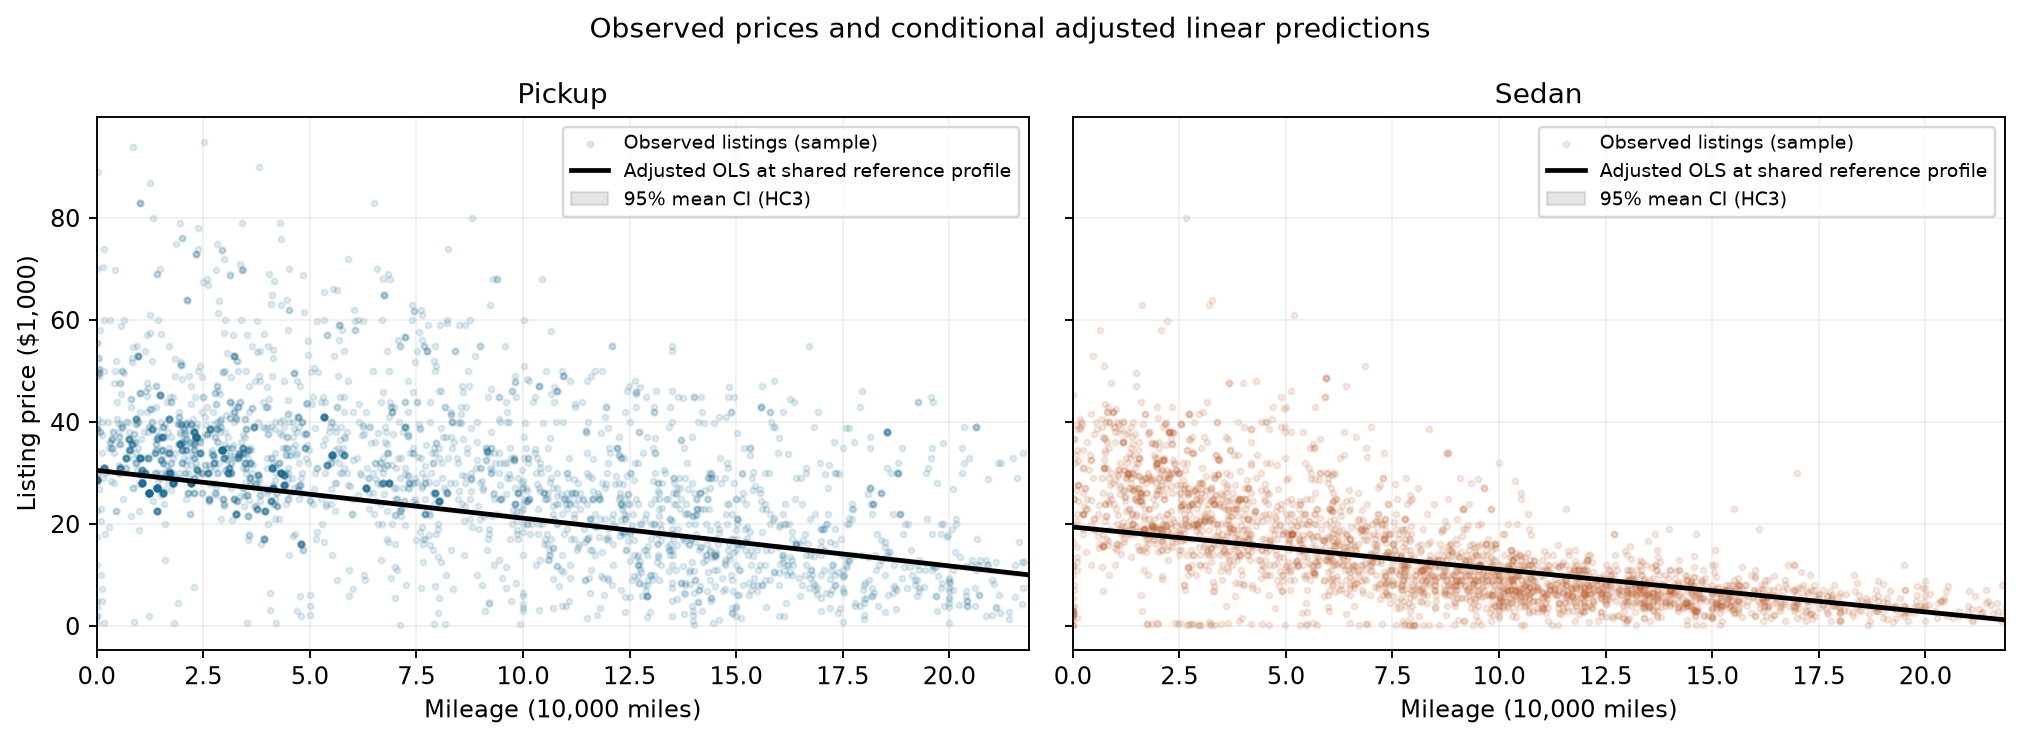
\includegraphics[width=.81\linewidth]{03_adjusted_linear_predictions.png}
\caption{Observed prices (3,000 sampled per type before the mileage display cutoff)
and adjusted fits for a seven-year-old Ford in good condition with automatic transmission
and front-wheel drive. Shading shows pointwise 95\% HC3 intervals for the mean.}
\label{fig:linear}
\end{figure}

\newpage

\subsection*{Linear model diagnostics}

We used Breusch--Pagan to test whether residual variance was constant across
the selected predictors. Jarque--Bera uses residual skewness and kurtosis to check
normality, an assumption for exact classical \(t\) inference along with independent
errors of constant variance. Both tests gave \(p<0.0001\). Their usual reference
distributions rely on independence, so repeated listings warrant caution.

HC3 allows unequal error variance and uses a large-sample approximation under
independence across listings. As a sensitivity check, VIN-clustered inference allows
errors to be correlated within known VINs and relies on independence across the
inferred groups. The adjusted fit improved in-sample \(R^2\) from 0.517 to 0.647.
The design had full rank (52 columns),
with an interaction variance inflation factor of 3.89. Mean sedan residuals went
from \negnum{\$2,025} at 80,000--100,000 miles to \posnum{\$4,047} at
200,000--220,000 miles, consistent with the flattening seen in Checkpoint~1.

\subsection*{The slope difference varies with mileage}

The joint HC3 Wald test asks whether all three quadratic coefficients are zero
together, the restriction that reduces the quadratic model to the linear one.
Using the same large-sample assumptions as the HC3 slope tests, it gave
\(\chi^2(3)=7{,}069.71\), \(p<0.0001\). Adjusted \(R^2\) increased from 0.646
to 0.699. In the quadratic fit, the sedan curve flattens more
sharply than the pickup curve. At 50,000 miles, the fitted pickup slope is
\$169 less negative than the sedan slope per 10,000 miles. At 100,000 miles,
the pickup slope is about \$157 more negative (Table~\ref{tab:local}).
The contrast is \(\delta+2\kappa m\), where \(\kappa\) is the coefficient on
\(m_i^2P_i\) in the quadratic model. It crosses zero near 76,000 miles.

\begin{table}[H]
\caption{Local quadratic slopes in dollars per 10,000 miles.}
\label{tab:local}
\small
\renewcommand{\arraystretch}{1.14}
\begin{tabular*}{\linewidth}{@{\extracolsep{\fill}}lrrrr@{}}
\toprule
\textbf{Mileage} & \textbf{Sedan} & \textbf{Pickup} & \textbf{Pickup minus sedan} &
\textbf{HC3 95\% CI for difference} \\
\midrule
50,000  & \negnum{864.01} & \negnum{695.22} & \posnum{168.79} &
  \confint{\posnum{135.82}}{\posnum{201.77}} \\
100,000 & \negnum{501.48} & \negnum{657.98} & \negnum{156.50} &
  \confint{\negnum{175.00}}{\negnum{138.00}} \\
150,000 & \negnum{138.95} & \negnum{620.75} & \negnum{481.80} &
  \confint{\negnum{502.64}}{\negnum{460.96}} \\
200,000 & \posnum{223.58} & \negnum{583.52} & \negnum{807.10} &
  \confint{\negnum{844.02}}{\negnum{770.17}} \\
\bottomrule
\end{tabular*}
\tabnote{Slopes are derivatives at the indicated mileage, scaled to 10,000-mile
units. Intervals are pointwise.}
\end{table}

At 200,000 miles the quadratic sedan derivative is positive. There are 1,033 sedans
in the 200,000--220,000-mile bin versus 9,996 in the 80,000--100,000-mile bin.
The fitted upturn calls for
checking functional form and vehicle mix in the upper tail before interpreting
that slope as a market pattern.

\subsection*{Performance on held-out vehicle groups}

The adjusted quadratic fit had the lowest test RMSE in every split and reduced
mean RMSE by \$633 (7.7\%) relative to adjusted linear OLS. It also improved
mean MAE and test \(R^2\) (Table~\ref{tab:validation}). At 100,000 miles its
pickup-minus-sedan dollar slope difference ranged from \negnum{\$181.89} to
\negnum{\$141.48} across the five training sets. The adjusted linear difference
also stayed negative, from \negnum{\$132.66} to \negnum{\$88.02}.

\begin{table}[H]
\caption{Test performance across five splits grouped by vehicle.}
\label{tab:validation}
\small
\renewcommand{\arraystretch}{1.14}
\begin{tabular*}{\linewidth}{@{\extracolsep{\fill}}lrrr@{}}
\toprule
\textbf{Model} & \textbf{MAE (\$)} & \textbf{RMSE (\$)} & \textbf{\(R^2\)} \\
\midrule
Unadjusted linear & \(6{,}757\pm114\) & \(9{,}535\pm138\) & \(0.519\pm0.009\) \\
Adjusted linear & \(5{,}557\pm81\) & \(8{,}187\pm67\) & \(0.645\pm0.005\) \\
Adjusted log-price & \(5{,}421\pm168\) & \(8{,}189\pm206\) & \(0.645\pm0.021\) \\
\textbf{Adjusted quadratic} & \(5{,}054\pm99\) & \(7{,}554\pm117\) &
  \(0.698\pm0.006\) \\
\bottomrule
\end{tabular*}
\tabnote{Entries are mean \(\pm\) standard deviation across the five splits. All
prediction errors use the original dollar scale. The log-price model estimates
its slope contrast in log-price units.}
\end{table}

\newpage

\subsection*{Sensitivity to cleaning, influence, and listing repetition}

Leverage and Cook's distance flagged 7,133 and 5,309 listings,
respectively. We refit the adjusted linear model with alternative cleaning rules,
after removing the top 1\% by Cook's distance, and with one listing per known VIN.

\begin{table}[H]
\caption{Selected sensitivity checks for the adjusted linear slope contrast.
Estimates and intervals are dollars per 10,000 miles.}
\label{tab:sensitivity}
\small
\renewcommand{\arraystretch}{1.16}
\begin{tabular*}{\linewidth}{@{\extracolsep{\fill}}lrrr@{}}
\toprule
\textbf{Sample rule} & \textbf{Listings} & \textbf{Pickup minus sedan} & \textbf{HC3 95\% CI} \\
\midrule
Checkpoint 1 bounds (primary) & 119,016 & \negnum{104.46} &
  \confint{\negnum{122.86}}{\negnum{86.07}} \\
Conservative used-vehicle subset & 113,459 & \negnum{116.92} &
  \confint{\negnum{133.24}}{\negnum{100.59}} \\
Remove top 1\% by Cook's distance & 117,825 & \negnum{132.91} &
  \confint{\negnum{149.63}}{\negnum{116.19}} \\
First listing per known VIN & 68,342 & \negnum{486.14} &
  \confint{\negnum{515.27}}{\negnum{457.01}} \\
Relax price and mileage ceilings & 119,073 & \negnum{101.12} &
  \confint{\negnum{119.95}}{\negnum{82.29}} \\
\bottomrule
\end{tabular*}
\tabnote{The conservative subset required at least \$1,000 and 1,000 miles,
age 1--30 years, and excluded listings marked new. The relaxed ceilings of
\$150,000 and 450,000 miles admitted 57 more listings. The VIN refit kept the
first row per plausible VIN and all rows without a usable VIN.}
\end{table}

All tested linear refits gave negative differences. Additional
checks varied the minimum price, minimum mileage, age, and mileage cap, and excluded
listings marked new. Keeping one listing per known VIN moved the estimate most and
reduced the pickup share from 34.0\% to 26.2\%. On the full sample, clustering by
VIN raised the standard error from \$9.39 to \$27.23 and widened the 95\% interval
to \negnum{\$157.84} through \negnum{\$51.08}. The 33,772 listings without usable
VINs entered as singletons, so some dependence may remain.

\section{Evaluation of the Original Hypothesis and Plan}

Checkpoint~1 found higher asking prices for pickups and flattening at higher
mileage. The new estimates show that higher price levels can coexist with
steeper adjusted dollar declines. The direction predicted in the proposal
appears at lower mileage in the quadratic fit. The adjusted linear model and
estimates at 100,000 and 150,000 miles challenge a consistently smaller decline.

Residual patterns and holdout performance favor revising the constant-slope
assumption. Our estimates describe how asking prices vary across listings on
Craigslist in April--May 2021. Trim, geography, seller characteristics, and
unrecorded condition can still confound that association.

\section{Next-Step Plan or Revision}

We will retain the dollar-based question and the linear benchmark, and revise the
main comparison to allow the mileage slope to vary.

\begin{enumerate}
\item Fit a type-specific mileage spline with flexible age adjustment. Check
overlap and compare fitted dollar changes over 10,000-mile intervals beginning
at 50,000, 100,000, and 150,000 miles, with clustered intervals.
\item To assess the effect of repeated vehicles, compare all listings and one
listing per VIN within the usable-VIN subset. Keep the earliest post per VIN,
using listing ID to break ties.
\item Compare models on matched grouped holdouts. Learn category pooling on
training data and report MAE, RMSE, and mean residual by vehicle type and
mileage band to check the ranges used in the final comparison.
\end{enumerate}


\newpage

\subsection*{Sources and verification}

\textbf{Dataset:} Austin Reese, Used Cars Dataset, Kaggle: \newline
\url{https://www.kaggle.com/datasets/austinreese/craigslist-carstrucks-data}.
Download details and checksum are recorded in \texttt{checkpoint1/data/source.json}.

\textbf{Project materials:} The \href{https://github.com/masikomamba/data_mining/blob/0ea7066/Team_research_Proposal.pdf}{team proposal} and
\href{https://github.com/masikomamba/data_mining/blob/0ea7066/checkpoint1/Checkpoint1_report.pdf}{Checkpoint 1 report}
document the original hypothesis and the cleaning rules.

\textbf{Analysis and verification:} The
\href{https://github.com/masikomamba/data_mining/blob/0ea7066/checkpoint2/Checkpoint1_with_Checkpoint2_ran.ipynb}{executed notebook} and
\href{https://github.com/masikomamba/data_mining/blob/0ea7066/checkpoint2/checkpoint2_outputs.zip}{results archive}
are from repository commit \texttt{0ea7066}. To reproduce the analysis, place
\texttt{vehicles.csv} beside the notebook or in its \texttt{data/} subdirectory
and run the Checkpoint~1 cells followed by the Checkpoint~2 cells. The final
cell exports the tables and figures. Export tables 01--04 cover the sample
and encoding, 05--15 the linear models and diagnostics, 16--19 curvature and
holdouts, and 20--21 sensitivity and validity limits.

\textbf{Statistical methods:} MacKinnon and White (1985),
\href{https://doi.org/10.1016/0304-4076(85)90158-7}{\emph{Journal of Econometrics}, 29(3), 305--325}
(heteroskedasticity-consistent covariance estimates). Duan (1983),
\href{https://doi.org/10.1080/01621459.1983.10478017}{\emph{Journal of the American Statistical Association}, 78(383), 605--610}
(smearing retransformation).

\end{document}
